\documentclass[11pt,a4paper]{article}
\usepackage[latin5]{inputenc}
\usepackage[english]{babel}
\usepackage{amsmath}
\usepackage{amsfonts}
\usepackage{amssymb}
\usepackage{graphicx,subfig}
\usepackage{placeins}
\author{Alexander Attinger, Yannic Kilcher}
\title{Report Blatt 3}

\begin{document}
\maketitle
\section{Exercise 1 Edge Detection}
As descriped in sheet one for the Laplacian, edges are usually denoted by strong change of intensity over short distances. Thus they can be detected by calculating

\subsection{Sobel Edge Detection}
The sobel operator is a specific filter convolved with the Image $P$. It is used to approximate the calculation of the gradient in x and y direction. To compute the gradient $G_{x}$ in x direction:

\[
\begin{array}{lcc}
G_{x} = & \left(\begin{array}{@{}ccc@{}}
                    -1 & 0 & 1 \\
                    -2 & 0 & 2 \\
                    -1 & 0 & 1
                  \end{array}\right) & *\quad P\\[15pt]
  
\end{array} 
\]

is used and for y direction $G_{y}$:

\[
\begin{array}{lcc}
G_{y} = & \left(\begin{array}{@{}ccc@{}}
                    -1 & -2 & -1 \\
                    0 & 0 & 0 \\
                    1 & 2 & 1
                  \end{array}\right)\quad *\quad P\\[15pt]
  
\end{array}
\]
 is used. OpenCV implements the Sobel function, i.e. it allows to calculate $G_{x} and G_{y}$. The gradient magnitude $G$ can be calculated in different ways, we used:
 \begin{equation}
 G = .5*\lvert G_{x}+G_{x}\rvert
 \end{equation}
 
We then implemented a simpel thresholding on $G$ to label pixels as Edge/background. As can be seen in the pictures, the detection works ok, at least for the human eye. Some points:
\begin{itemize}
\item Threshold value had to be adjusted for each picture individually
\item In all pictures it is also hard to judge by eye, which part actually are edges and which are not
\item In images with a clear foreground/background edge detection on the foreground object works fairly well (e.g. Butterfly)
\item images with no clear distinction suc
\end{itemize}
\begin{figure}%
\centering
\subfloat[][Original Image]{\includegraphics[scale=.3]{res/striped-lines.png}}
\quad
\subfloat[][Phase Image]{\includegraphics[scale=.3]{res/a1phase.png}}
\quad
\subfloat[][Log Magnitude Image]{\includegraphics[scale=.3]{res/a1mag.png}}
\quad

\caption{Fourier transformation of a stripe pattern.}%
\label{fig:a1a}%
\end{figure}

\subsection{Canny Edge Detection}


\begin{figure}%
\centering
\subfloat[][Original Image 1]{\includegraphics[scale=.7]{res/h.png}}
\quad
\subfloat[][Original Image 2]{\includegraphics[scale=.7]{res/v.png}}
\quad
\subfloat[][Result after convolution]{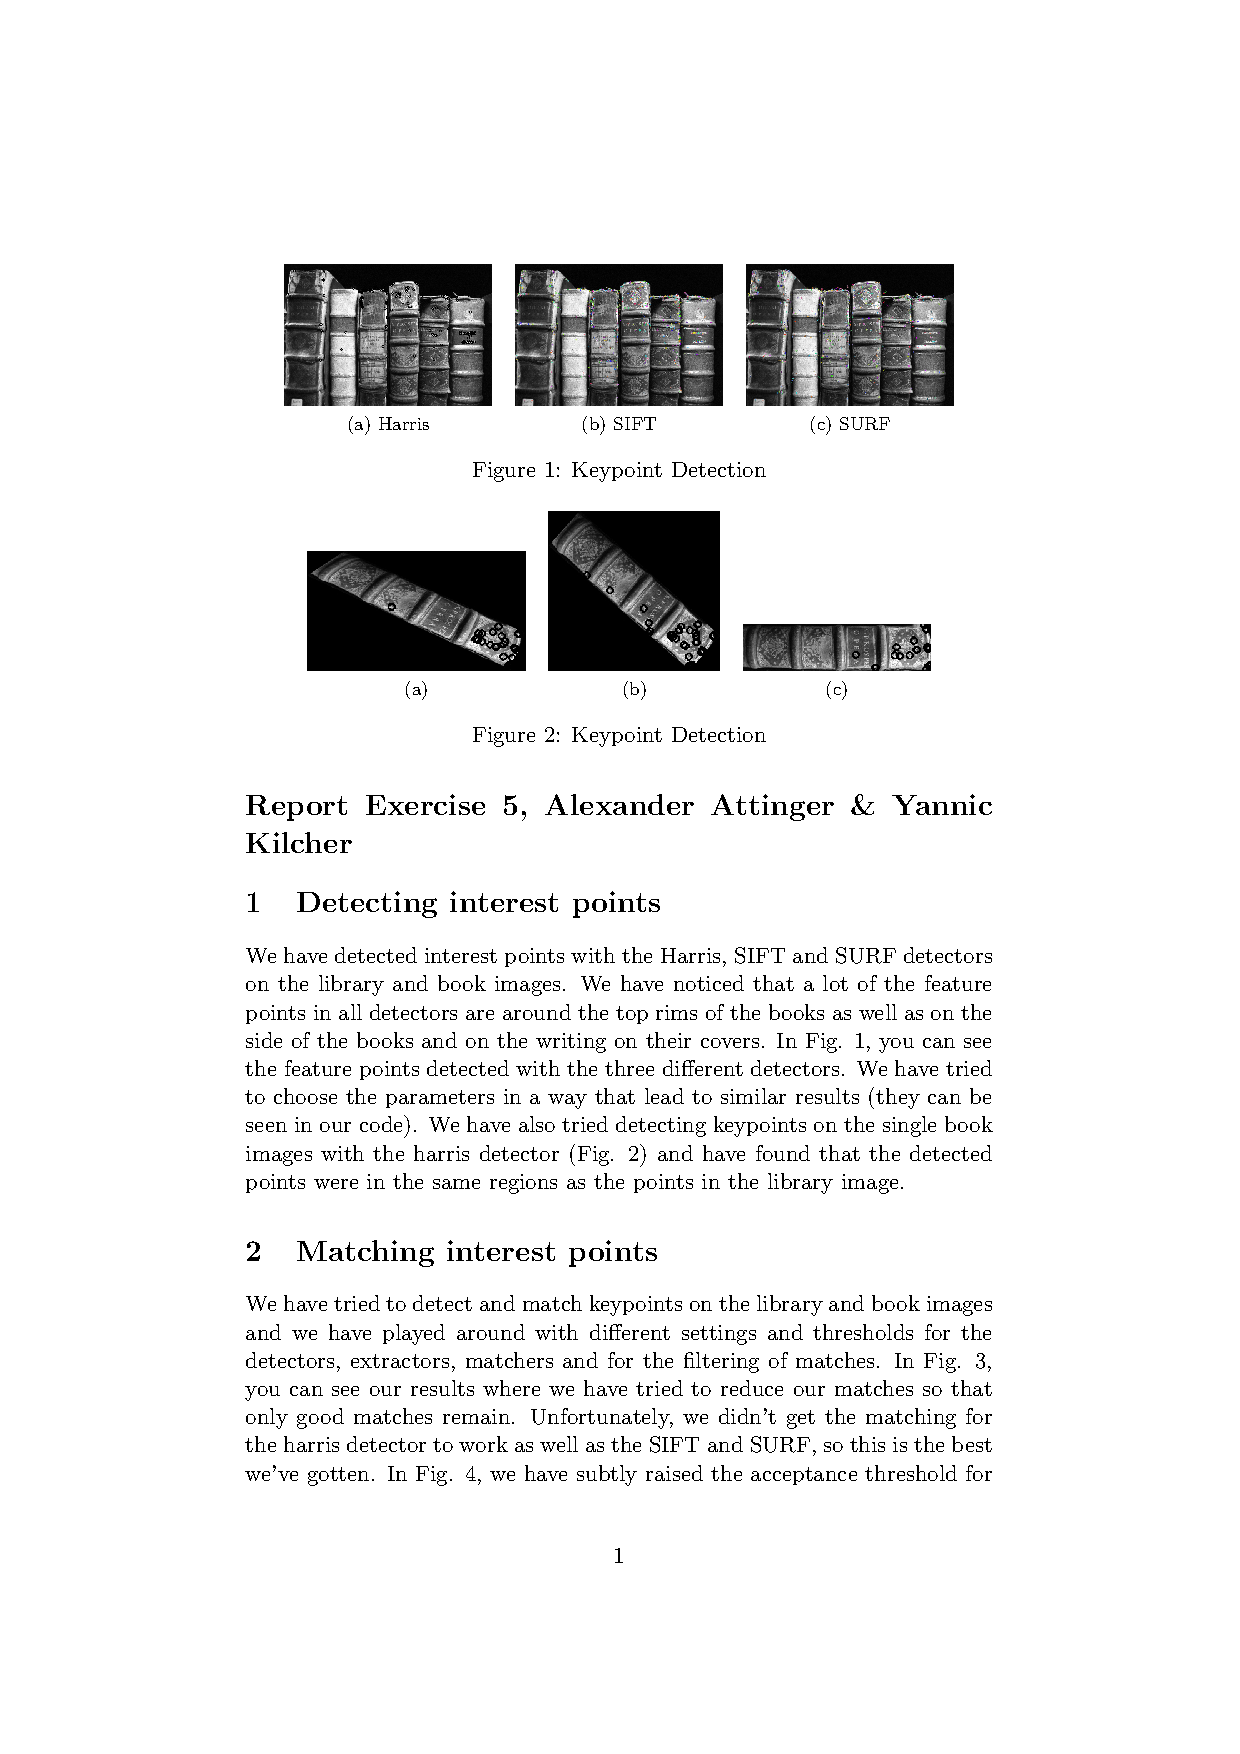
\includegraphics[scale=.7]{res/a2.png}}
\quad

\caption{Spatial convolution of two images.}%
\label{fig:a1b}%
\end{figure}

\subsection{Comparison}



\FloatBarrier

\section{Excercise 2}

\end{document}
